% Options for packages loaded elsewhere
% Options for packages loaded elsewhere
\PassOptionsToPackage{unicode}{hyperref}
\PassOptionsToPackage{hyphens}{url}
%
\documentclass[
  14pt,
  ignorenonframetext,
  aspectratio=169,
]{beamer}
\newif\ifbibliography
\usepackage{pgfpages}
\setbeamertemplate{caption}[numbered]
\setbeamertemplate{caption label separator}{: }
\setbeamercolor{caption name}{fg=normal text.fg}
\beamertemplatenavigationsymbolsempty
% remove section numbering
\setbeamertemplate{part page}{
  \centering
  \begin{beamercolorbox}[sep=16pt,center]{part title}
    \usebeamerfont{part title}\insertpart\par
  \end{beamercolorbox}
}
\setbeamertemplate{section page}{
  \centering
  \begin{beamercolorbox}[sep=12pt,center]{section title}
    \usebeamerfont{section title}\insertsection\par
  \end{beamercolorbox}
}
\setbeamertemplate{subsection page}{
  \centering
  \begin{beamercolorbox}[sep=8pt,center]{subsection title}
    \usebeamerfont{subsection title}\insertsubsection\par
  \end{beamercolorbox}
}
% Prevent slide breaks in the middle of a paragraph
\widowpenalties 1 10000
\raggedbottom
\usepackage{iftex}
\ifPDFTeX
  \usepackage[T1]{fontenc}
  \usepackage[utf8]{inputenc}
  \usepackage{textcomp} % provide euro and other symbols
\else % if luatex or xetex
  \usepackage{unicode-math} % this also loads fontspec
  \defaultfontfeatures{Scale=MatchLowercase}
  \defaultfontfeatures[\rmfamily]{Ligatures=TeX,Scale=1}
\fi
\usepackage{lmodern}

\usetheme[]{monash}
\ifPDFTeX\else
  % xetex/luatex font selection
\fi
% Use upquote if available, for straight quotes in verbatim environments
\IfFileExists{upquote.sty}{\usepackage{upquote}}{}
\IfFileExists{microtype.sty}{% use microtype if available
  \usepackage[]{microtype}
  \UseMicrotypeSet[protrusion]{basicmath} % disable protrusion for tt fonts
}{}
\makeatletter
\@ifundefined{KOMAClassName}{% if non-KOMA class
  \IfFileExists{parskip.sty}{%
    \usepackage{parskip}
  }{% else
    \setlength{\parindent}{0pt}
    \setlength{\parskip}{6pt plus 2pt minus 1pt}}
}{% if KOMA class
  \KOMAoptions{parskip=half}}
\makeatother

\usepackage{color}
\usepackage{fancyvrb}
\newcommand{\VerbBar}{|}
\newcommand{\VERB}{\Verb[commandchars=\\\{\}]}
\DefineVerbatimEnvironment{Highlighting}{Verbatim}{commandchars=\\\{\}}
% Add ',fontsize=\small' for more characters per line
\usepackage{framed}
\definecolor{shadecolor}{RGB}{248,248,248}
\newenvironment{Shaded}{\begin{snugshade}}{\end{snugshade}}
\newcommand{\AlertTok}[1]{\textcolor[rgb]{0.94,0.16,0.16}{#1}}
\newcommand{\AnnotationTok}[1]{\textcolor[rgb]{0.56,0.35,0.01}{\textbf{\textit{#1}}}}
\newcommand{\AttributeTok}[1]{\textcolor[rgb]{0.13,0.29,0.53}{#1}}
\newcommand{\BaseNTok}[1]{\textcolor[rgb]{0.00,0.00,0.81}{#1}}
\newcommand{\BuiltInTok}[1]{#1}
\newcommand{\CharTok}[1]{\textcolor[rgb]{0.31,0.60,0.02}{#1}}
\newcommand{\CommentTok}[1]{\textcolor[rgb]{0.56,0.35,0.01}{\textit{#1}}}
\newcommand{\CommentVarTok}[1]{\textcolor[rgb]{0.56,0.35,0.01}{\textbf{\textit{#1}}}}
\newcommand{\ConstantTok}[1]{\textcolor[rgb]{0.56,0.35,0.01}{#1}}
\newcommand{\ControlFlowTok}[1]{\textcolor[rgb]{0.13,0.29,0.53}{\textbf{#1}}}
\newcommand{\DataTypeTok}[1]{\textcolor[rgb]{0.13,0.29,0.53}{#1}}
\newcommand{\DecValTok}[1]{\textcolor[rgb]{0.00,0.00,0.81}{#1}}
\newcommand{\DocumentationTok}[1]{\textcolor[rgb]{0.56,0.35,0.01}{\textbf{\textit{#1}}}}
\newcommand{\ErrorTok}[1]{\textcolor[rgb]{0.64,0.00,0.00}{\textbf{#1}}}
\newcommand{\ExtensionTok}[1]{#1}
\newcommand{\FloatTok}[1]{\textcolor[rgb]{0.00,0.00,0.81}{#1}}
\newcommand{\FunctionTok}[1]{\textcolor[rgb]{0.13,0.29,0.53}{\textbf{#1}}}
\newcommand{\ImportTok}[1]{#1}
\newcommand{\InformationTok}[1]{\textcolor[rgb]{0.56,0.35,0.01}{\textbf{\textit{#1}}}}
\newcommand{\KeywordTok}[1]{\textcolor[rgb]{0.13,0.29,0.53}{\textbf{#1}}}
\newcommand{\NormalTok}[1]{#1}
\newcommand{\OperatorTok}[1]{\textcolor[rgb]{0.81,0.36,0.00}{\textbf{#1}}}
\newcommand{\OtherTok}[1]{\textcolor[rgb]{0.56,0.35,0.01}{#1}}
\newcommand{\PreprocessorTok}[1]{\textcolor[rgb]{0.56,0.35,0.01}{\textit{#1}}}
\newcommand{\RegionMarkerTok}[1]{#1}
\newcommand{\SpecialCharTok}[1]{\textcolor[rgb]{0.81,0.36,0.00}{\textbf{#1}}}
\newcommand{\SpecialStringTok}[1]{\textcolor[rgb]{0.31,0.60,0.02}{#1}}
\newcommand{\StringTok}[1]{\textcolor[rgb]{0.31,0.60,0.02}{#1}}
\newcommand{\VariableTok}[1]{\textcolor[rgb]{0.00,0.00,0.00}{#1}}
\newcommand{\VerbatimStringTok}[1]{\textcolor[rgb]{0.31,0.60,0.02}{#1}}
\newcommand{\WarningTok}[1]{\textcolor[rgb]{0.56,0.35,0.01}{\textbf{\textit{#1}}}}

\usepackage{longtable,booktabs,array}
\newcounter{none} % for unnumbered tables
\usepackage{calc} % for calculating minipage widths
\usepackage{caption}
% Make caption package work with longtable
\makeatletter
\def\fnum@table{\tablename~\thetable}
\makeatother
\usepackage{graphicx}
\makeatletter
\newsavebox\pandoc@box
\newcommand*\pandocbounded[1]{% scales image to fit in text height/width
  \sbox\pandoc@box{#1}%
  \Gscale@div\@tempa{\textheight}{\dimexpr\ht\pandoc@box+\dp\pandoc@box\relax}%
  \Gscale@div\@tempb{\linewidth}{\wd\pandoc@box}%
  \ifdim\@tempb\p@<\@tempa\p@\let\@tempa\@tempb\fi% select the smaller of both
  \ifdim\@tempa\p@<\p@\scalebox{\@tempa}{\usebox\pandoc@box}%
  \else\usebox{\pandoc@box}%
  \fi%
}
% Set default figure placement to htbp
\def\fps@figure{htbp}
\makeatother





\setlength{\emergencystretch}{3em} % prevent overfull lines

\providecommand{\tightlist}{%
  \setlength{\itemsep}{0pt}\setlength{\parskip}{0pt}}



 


% Colors
\definecolor{shadecolor}{RGB}{225,225,225}
\setbeamercolor{description item}{fg=Orange}
\definecolor{MonashBlue}{RGB}{66,109,152}
\definecolor{burntorange}{rgb}{0.8, 0.33, 0.0}

% Packages
\usepackage{amsmath, bm, amssymb, amsthm, mathrsfs,pifont}
\usepackage{url}
\usepackage{multirow, booktabs, float, textcmds, siunitx}
\usepackage{bm,booktabs,animate,ragged2e,multicol,microtype,hyperref}
\usepackage{fontawesome5}

% Figures
\graphicspath{{figs/}}

% Fonts
\fontsize{13}{15}\sf
\setbeamerfont{title}{series=\bfseries,parent=structure,size=\fontsize{24}{24}}
\ifcsname Shaded\endcsname
  \definecolor{shadecolor}{RGB}{225,225,225}
  \renewenvironment{Shaded}{\vspace*{0.15cm}\color{black}\fontsize{10}{10}\sf\begin{snugshade}\color{black}}{\end{snugshade}}
\fi

% gt dependencies
\usepackage{longtable,caption,setspace}
\captionsetup{font={small,stretch=0.80}}

% My definitions

\def\E{\text{E}}
\def\V{\text{Var}}
\def\up#1{\raisebox{-0.3cm}{#1}}
\def\pred#1#2#3{\hat{#1}_{#2|#3}}
\def\damped{$_\text{d}$}
\def\h+{h_{m}^{+}}
\def\str#1{\rlap{#1}\textcolor{red}{\rule{1cm}{0.1cm}}}

\def\st#1{\rlap{#1}\textcolor{red}{\rule{1cm}{0.1cm}}}
\def\bY{\bm{y}}
\def\by{\bm{y}}
\def\bS{\bm{S}}
\def\bI{\text{\rm\textbf{I}}}
\def\bbeta{\bm{\beta}}
\def\bSigma{\bm{\Sigma}}
\def\bW{\bm{\Sigma}}
\def\Var{\text{Var}}
\def\var{\text{Var}}
\def\bOmega{\bm{\Omega}}
\def\bLambda{\bm{\Lambda}}
\let\mc\multicolumn
\def\hl{\color[RGB]{230, 172, 0}}

\def\forecast{\begin{alertblock}{}\fontsize{10}{11}\sf
 A forecast is an estimate of the probability distribution of a variable to be observed in the future.
\end{alertblock}}

\def\simfutures{\begin{textblock}{2.9}(12.8,7.7)
\begin{block}{}\fontsize{10}{11}\sf
Simulated futures from an ETS model
\end{block}\end{textblock}}

\setbeamertemplate{title page}
{\placefig{0}{-0.5}{width=1.01\paperwidth,height=1.45\paperheight}{africa1.jpg}
\begin{textblock}{8.5}(.5,0.2)
  \raggedright\fontsize{20}{20}\selectfont\bfseries\sffamily\textcolor{white}{\inserttitle}\\[0.2cm]
  \fontsize{12}{12}\selectfont\bfseries\sffamily\textcolor{white}{\insertsubtitle}
  \end{textblock}
\placefig{.5}{6.2}{width=2.4cm}{tsibble.png}
\placefig{2.9}{6.2}{width=2.4cm}{feasts.png}
\placefig{5.3}{6.2}{width=2.4cm}{fable.png}
\begin{textblock}{7.5}(10.6,-.1)
  {\fontsize{9}{9}\sf\color{white}https://workshop.f4sg.org/africast/}
\end{textblock}
}

% Tikz plots
\usepackage{tikz}
\usetikzlibrary{trees,shapes,arrows,matrix,shadows,positioning,calc}
\tikzstyle{decision} = [diamond, draw, fill=blue!20,
    text width=4.5em, text badly centered, node distance=4cm, inner sep=0pt]
\tikzstyle{block} = [rectangle, draw, fill=blue!20,
    text width=5cm, text centered, rounded corners, minimum height=4em]
\tikzstyle{line} = [draw, thick, -latex']
\tikzstyle{cloud} = [draw, ellipse,fill=red!20, node distance=3cm,
    minimum height=2em, text centered]
\tikzstyle{connector} = [->,thick]

\tikzset{
  basic/.style  = {draw, text width=2cm, font=\sffamily, rectangle},
  root/.style   = {basic, text width=3cm, rounded corners=2pt, thin, align=center, fill=red!30},
  level 2a/.style = {basic, rounded corners=2pt, thin,align=center, fill=blue!50, text width=7em},
  level 2b/.style = {basic, rounded corners=2pt, thin,align=center, fill=green!50, text width=7em},
  level 3a/.style = {basic, rounded corners=2pt, thin, align=center, fill=blue!30, text width=4em},
  level 3b/.style = {basic, rounded corners=2pt, thin, align=center, fill=green!30, text width=4em},
  level 4a/.style = {basic, rounded corners=2pt, thin, align=left, fill=blue!10, text width=3.5em},
  level 4b/.style = {basic, rounded corners=2pt, thin, align=left, fill=green!10, text width=3.5em}
}

% % BIBLIOGRAPHIES
% \usepackage[style=authoryear,bibencoding=utf8,minnames=1,maxnames=4, maxbibnames=99,natbib=true,dashed=false,terseinits=true,giveninits=true,uniquename=false,uniquelist=false,labeldate=true,doi=false, isbn=false, natbib=true,backend=biber]{biblatex}

% \DeclareFieldFormat{url}{\url{#1}}
% \DeclareFieldFormat[article]{pages}{#1}
% \DeclareFieldFormat[inproceedings]{pages}{\lowercase{pp.}#1}
% \DeclareFieldFormat[incollection]{pages}{\lowercase{pp.}#1}
% \DeclareFieldFormat[article]{volume}{\mkbibbold{#1}}
% \DeclareFieldFormat[article]{number}{\mkbibparens{#1}}
% \DeclareFieldFormat[article]{title}{\MakeCapital{#1}}
% \DeclareFieldFormat[article]{url}{}
% \DeclareFieldFormat[Techreport]{Url}{}
% \DeclareFieldFormat[book]{url}{}
% \DeclareFieldFormat[inbook]{url}{}
% \DeclareFieldFormat[incollection]{url}{}
% \DeclareFieldFormat[inproceedings]{url}{}
% \DeclareFieldFormat[inproceedings]{title}{#1}
% \DeclareFieldFormat{shorthandwidth}{#1}
% %\DeclareFieldFormat{extrayear}{}
% % No dot before number of articles
% \usepackage{xpatch}
% \xpatchbibmacro{volume+number+eid}{\setunit*{\adddot}}{}{}{}
% % Remove In: for an article.
% \renewbibmacro{in:}{%
%   \ifentrytype{article}{}{%
%   \printtext{\bibstring{in}\intitlepunct}}}

% \AtEveryBibitem{\clearfield{month}}
% \AtEveryCitekey{\clearfield{month}}
% \AtBeginBibliography{\fontsize{11}{11}\sf}
\setbeamertemplate{frametitle continuation}{}
\makeatletter
\@ifpackageloaded{caption}{}{\usepackage{caption}}
\AtBeginDocument{%
\ifdefined\contentsname
  \renewcommand*\contentsname{Table of contents}
\else
  \newcommand\contentsname{Table of contents}
\fi
\ifdefined\listfigurename
  \renewcommand*\listfigurename{List of Figures}
\else
  \newcommand\listfigurename{List of Figures}
\fi
\ifdefined\listtablename
  \renewcommand*\listtablename{List of Tables}
\else
  \newcommand\listtablename{List of Tables}
\fi
\ifdefined\figurename
  \renewcommand*\figurename{Figure}
\else
  \newcommand\figurename{Figure}
\fi
\ifdefined\tablename
  \renewcommand*\tablename{Table}
\else
  \newcommand\tablename{Table}
\fi
}
\@ifpackageloaded{float}{}{\usepackage{float}}
\floatstyle{ruled}
\@ifundefined{c@chapter}{\newfloat{codelisting}{h}{lop}}{\newfloat{codelisting}{h}{lop}[chapter]}
\floatname{codelisting}{Listing}
\newcommand*\listoflistings{\listof{codelisting}{List of Listings}}
\makeatother
\makeatletter
\makeatother
\makeatletter
\@ifpackageloaded{caption}{}{\usepackage{caption}}
\@ifpackageloaded{subcaption}{}{\usepackage{subcaption}}
\makeatother

\usepackage{bookmark}
\IfFileExists{xurl.sty}{\usepackage{xurl}}{} % add URL line breaks if available
\urlstyle{same}
% fallback for those not using the hyperref driver hyperxmp:
\makeatletter
\@ifundefined{xmpquote}{\newcommand{\xmpquote}[1]{#1}}{}
\makeatother
\hypersetup{
  pdftitle={Africast-Time Series Analysis \& Forecasting Using R},
  hidelinks,
  pdfcreator={LaTeX via pandoc}}


\title{\texorpdfstring{Africast-Time Series Analysis \& Forecasting
Using R}{Africast-Time Series Analysis \& Forecasting Using R}}
\subtitle{\texorpdfstring{9. Basic training and test
accuracy}{9. Basic training and test accuracy}}
\author{}
\date{27 November 2025}

\begin{document}
\frame{\titlepage}


\begin{frame}{Outline}
\protect\phantomsection\label{outline}
\vspace*{0.7cm}\tableofcontents
\end{frame}

\section{Evaluating forecast
accuracy}\label{evaluating-forecast-accuracy}

\begin{frame}{Evaluate forecast accuracy}
\protect\phantomsection\label{evaluate-forecast-accuracy}
\begin{itemize}
\tightlist
\item
  In order to evaluate the performance of a forecasting model, we
  compute its forecast accuracy.
\item
  Forecast accuracy is compared by measuring errors based on the test
  set.
\item
  Ideally it should allow comparing benefits from improved accuracy with
  the cost of obtaining the improvement.
\end{itemize}
\end{frame}

\begin{frame}{Evaluate forecast accuracy- Business impact}
\protect\phantomsection\label{evaluate-forecast-accuracy--business-impact}
\begin{itemize}
\tightlist
\item
  We should be choosing forecast models that lead to better business
  decisions

  \begin{itemize}
  \tightlist
  \item
    least staffing costs, least emission, highest service level, least
    stock-out, least inventory, fastest response, least change in
    planing, for example.
  \end{itemize}
\item
  However, this is not always easy to obtain, therefore we might simply
  use methods that provide the most accurate forecast.
\end{itemize}
\end{frame}

\begin{frame}{In-sample (training) vs.~out-of-sample (test)}
\protect\phantomsection\label{in-sample-training-vs.-out-of-sample-test}
\begin{itemize}
\tightlist
\item
  Fitting and its residual are not a reliable indication of forecast
  accuracy
\item
  A model which fits the training data well will not necessarily
  forecast well
\item
  A perfect fit can always be obtained by using a model with enough
  parameters
\item
  Over-fitting a model to data is just as bad as failing to identify a
  systematic pattern in the data
\end{itemize}
\end{frame}

\begin{frame}{Forecast accuracy evaluation using test sets}
\protect\phantomsection\label{forecast-accuracy-evaluation-using-test-sets}
\begin{itemize}
\tightlist
\item
  We mimic the real life situation
\item
  We pretend we don't know some part of data (new data)
\item
  It must not be used for \emph{any} aspect of model training
\item
  Forecast accuracy is computed only based on the test set
\end{itemize}
\end{frame}

\begin{frame}{Training and test sets}
\protect\phantomsection\label{training-and-test-sets}
\pandocbounded{\includegraphics[keepaspectratio]{05_accuracy_basic_files/figure-beamer/traintest-1.pdf}}
\end{frame}

\section{Evaluating point forecast
accuracy}\label{evaluating-point-forecast-accuracy}

\begin{frame}{Forecast errors}
\protect\phantomsection\label{forecast-errors}
Forecast ``error'': the difference between an observed value and its
forecast. \[
  e_{T+h} = y_{T+h} - \hat{y}_{T+h|T},
\] where the training data is given by \(\{y_1,\dots,y_T\}\)
\end{frame}

\begin{frame}[fragile]{Measures of forecast accuracy}
\protect\phantomsection\label{measures-of-forecast-accuracy}
\fontsize{11}{12}\sf

\begin{Shaded}
\begin{Highlighting}[]
\NormalTok{beer\_fit }\OtherTok{\textless{}{-}}\NormalTok{ aus\_production }\SpecialCharTok{|\textgreater{}}
  \FunctionTok{filter}\NormalTok{(}\FunctionTok{between}\NormalTok{(}\FunctionTok{year}\NormalTok{(Quarter), }\DecValTok{1992}\NormalTok{, }\DecValTok{2007}\NormalTok{)) }\SpecialCharTok{|\textgreater{}}
  \FunctionTok{model}\NormalTok{(}
    \AttributeTok{snaive =} \FunctionTok{SNAIVE}\NormalTok{(Beer),}
    \AttributeTok{mean =} \FunctionTok{MEAN}\NormalTok{(Beer)}
\NormalTok{  )}
\NormalTok{beer\_fit }\SpecialCharTok{|\textgreater{}}
  \FunctionTok{forecast}\NormalTok{(}\AttributeTok{h =} \StringTok{"3 years"}\NormalTok{) }\SpecialCharTok{|\textgreater{}}
  \FunctionTok{autoplot}\NormalTok{(aus\_production, }\AttributeTok{level =} \ConstantTok{NULL}\NormalTok{) }\SpecialCharTok{+}
  \FunctionTok{labs}\NormalTok{(}\AttributeTok{title =}\StringTok{"Forecasts for quarterly beer production"}\NormalTok{,}
       \AttributeTok{x =}\StringTok{"Year"}\NormalTok{, }\AttributeTok{y =}\StringTok{"Megalitres"}\NormalTok{) }\SpecialCharTok{+}
  \FunctionTok{guides}\NormalTok{(}\AttributeTok{colour =} \FunctionTok{guide\_legend}\NormalTok{(}\AttributeTok{title =} \StringTok{"Forecast"}\NormalTok{))}
\end{Highlighting}
\end{Shaded}
\end{frame}

\begin{frame}{Measures of forecast accuracy}
\protect\phantomsection\label{measures-of-forecast-accuracy-1}
\pandocbounded{\includegraphics[keepaspectratio]{05_accuracy_basic_files/figure-beamer/beer-fc-1-1.pdf}}
\end{frame}

\begin{frame}{Measures of forecast accuracy}
\protect\phantomsection\label{measures-of-forecast-accuracy-2}
\begin{tabular}{rl}
$y_{T+h}=$ & $(T+h)$th observation, $h=1,\dots,H$ \\
$\pred{y}{T+h}{T}=$ & its forecast based on data up to time $T$. \\
$e_{T+h} =$  & $y_{T+h} - \pred{y}{T+h}{T}$
\end{tabular}

\begin{block}{}\vspace*{-0.7cm}
\begin{align*}
\text{MAE} &= \text{mean}(|e_{T+h}|) \\[-0.2cm]
\text{MSE} &= \text{mean}(e_{T+h}^2) \qquad
&&\text{RMSE} &= \sqrt{\text{mean}(e_{T+h}^2)} \\[-0.1cm]
\text{MAPE} &= 100\text{mean}(|e_{T+h}|/ |y_{T+h}|)
\end{align*}\vspace*{-0.9cm}
\end{block}
\pause

\begin{itemize}
\tightlist
\item
  MAE, MSE, RMSE are all scale dependent.
\item
  MAPE is scale independent but is only sensible if \(y_t\gg 0\) for all
  \(t\), and \(y\) has a natural zero.
\end{itemize}
\end{frame}

\begin{frame}{Measures of forecast accuracy}
\protect\phantomsection\label{measures-of-forecast-accuracy-3}
\fontsize{13}{15}\sf

\begin{block}{Mean Absolute Scaled Error}
$$
  \text{MASE} = \text{mean}(|e_{T+h}|/Q)
$$
\end{block} \pause

\begin{itemize}
\tightlist
\item
  For non-seasonal series, scale uses naïve forecasts:
\end{itemize}

\centerline{$Q = \frac{1}{T-1}\displaystyle\sum_{t=2}^T |y_{t}-y_{t-1}|$}

\begin{itemize}
\tightlist
\item
  For seasonal series, scale uses seasonal naïve forecasts:
\end{itemize}

\centerline{$Q = \frac{1}{T-m}\displaystyle\sum_{t=m+1}^T |y_{t}-y_{t-m}|$}
\rightline{where $m$ is the seasonal frequency}\pause

Proposed by Hyndman and Koehler (IJF, 2006).
\end{frame}

\begin{frame}{Measures of forecast accuracy}
\protect\phantomsection\label{measures-of-forecast-accuracy-4}
\fontsize{13}{15}\sf

\begin{block}{Root Mean Squared Scaled Error}
$$
  \text{RMSSE} = \sqrt{\text{mean}(e^2_{T+h}/Q)}
$$
\end{block}

\begin{itemize}
\tightlist
\item
  For non-seasonal series, scale uses naïve forecasts:
\end{itemize}

\centerline{$Q = \frac{1}{T-1}\displaystyle\sum_{t=2}^T (y_{t}-y_{t-1})^2$}

\begin{itemize}
\tightlist
\item
  For seasonal series, scale uses seasonal naïve forecasts:
\end{itemize}

\centerline{$Q = \frac{1}{T-m}\displaystyle\sum_{t=m+1}^T (y_{t}-y_{t-m})^2$}
\rightline{where $m$ is the seasonal frequencyq}

Proposed by Hyndman and Koehler (IJF, 2006).
\end{frame}

\begin{frame}[fragile]{Measures of forecast accuracy}
\protect\phantomsection\label{measures-of-forecast-accuracy-5}
\fontsize{9.8}{10}\sf

\begin{Shaded}
\begin{Highlighting}[]
\NormalTok{beer\_fc }\OtherTok{\textless{}{-}} \FunctionTok{forecast}\NormalTok{(beer\_fit, }\AttributeTok{h =} \StringTok{"3 years"}\NormalTok{)}
\FunctionTok{accuracy}\NormalTok{(beer\_fc, aus\_production)}
\end{Highlighting}
\end{Shaded}

\begin{verbatim}
# A tibble: 2 x 10
  .model .type    ME  RMSE   MAE   MPE  MAPE  MASE RMSSE    ACF1
  <chr>  <chr> <dbl> <dbl> <dbl> <dbl> <dbl> <dbl> <dbl>   <dbl>
1 mean   Test  -13.8  38.4  34.8 -3.97  8.28 2.20  1.96  -0.0691
2 snaive Test    5.2  14.3  13.4  1.15  3.17 0.847 0.729  0.132 
\end{verbatim}
\end{frame}

\section{Evaluating distributional forecast
accuracy}\label{evaluating-distributional-forecast-accuracy}

\begin{frame}{Prediction interval accuracy using winkler score}
\protect\phantomsection\label{prediction-interval-accuracy-using-winkler-score}
Winkler proposed a scoring method to enable comparisons between
prediction intervals:

\begin{itemize}
\tightlist
\item
  it takes account of both coverage and width of the intervals.
\end{itemize}

\begin{block}{Winkler score}
\begin{align*}
  W(l_t,u_t,y_t) =
    \begin{cases}
      u_t-l_t & \text{if $l_t < y_t <u_t$}\\
      (u_t-l_t)+ \frac{2}{\alpha}(l_t-y_t) & \text{if $y_t < l_t$}\\
      (u_t-l_t) + \frac{2}{\alpha}(y_t-u_t) & \text{if $y_t > u_t$}
    \end{cases}       
\end{align*}
\end{block}
\end{frame}

\begin{frame}[fragile]{Prediction interval accuracy}
\protect\phantomsection\label{prediction-interval-accuracy}
\fontsize{11}{12}\sf

\begin{Shaded}
\begin{Highlighting}[]
  \CommentTok{\# Compute interval accuracy}
\NormalTok{beer\_fc }\SpecialCharTok{|\textgreater{}} \FunctionTok{accuracy}\NormalTok{(aus\_production,}
   \AttributeTok{measures =}\NormalTok{ interval\_accuracy\_measures) }
\end{Highlighting}
\end{Shaded}

\begin{verbatim}
# A tibble: 2 x 5
  .model .type winkler pinball scaled_pinball
  <chr>  <chr>   <dbl>   <dbl>          <dbl>
1 mean   Test    174.     8.67         0.274 
2 snaive Test     86.3    3.10         0.0980
\end{verbatim}
\end{frame}

\begin{frame}{Quantile score}
\protect\phantomsection\label{quantile-score}
\begin{block}{Quantile score}
\begin{align*}
  Q_{p,t} = 
    \begin{cases}
    2(1 - p) \big(f_{p,t} - y_{t}\big), & \text{if $y_{t} < f_{p,t}$}\\
    2p \big(y_{t} - f_{p,t}\big), & \text{if $y_{t} \ge f_{p,t}$} 
    \end{cases}
\end{align*}
\end{block}
\end{frame}

\begin{frame}{Continuous Ranked Probability Score (CRPS)}
\protect\phantomsection\label{continuous-ranked-probability-score-crps}
\[\large \text{CRPS} = \text{mean}(p_j),\]

where

\[p_j = \int_{-\infty}^{\infty} \left(G_j(x) - F_j(x)\right)^2dx,\]
\end{frame}

\begin{frame}{Continuous Ranked Probability Score (CRPS)}
\protect\phantomsection\label{continuous-ranked-probability-score-crps-1}
\begin{center}
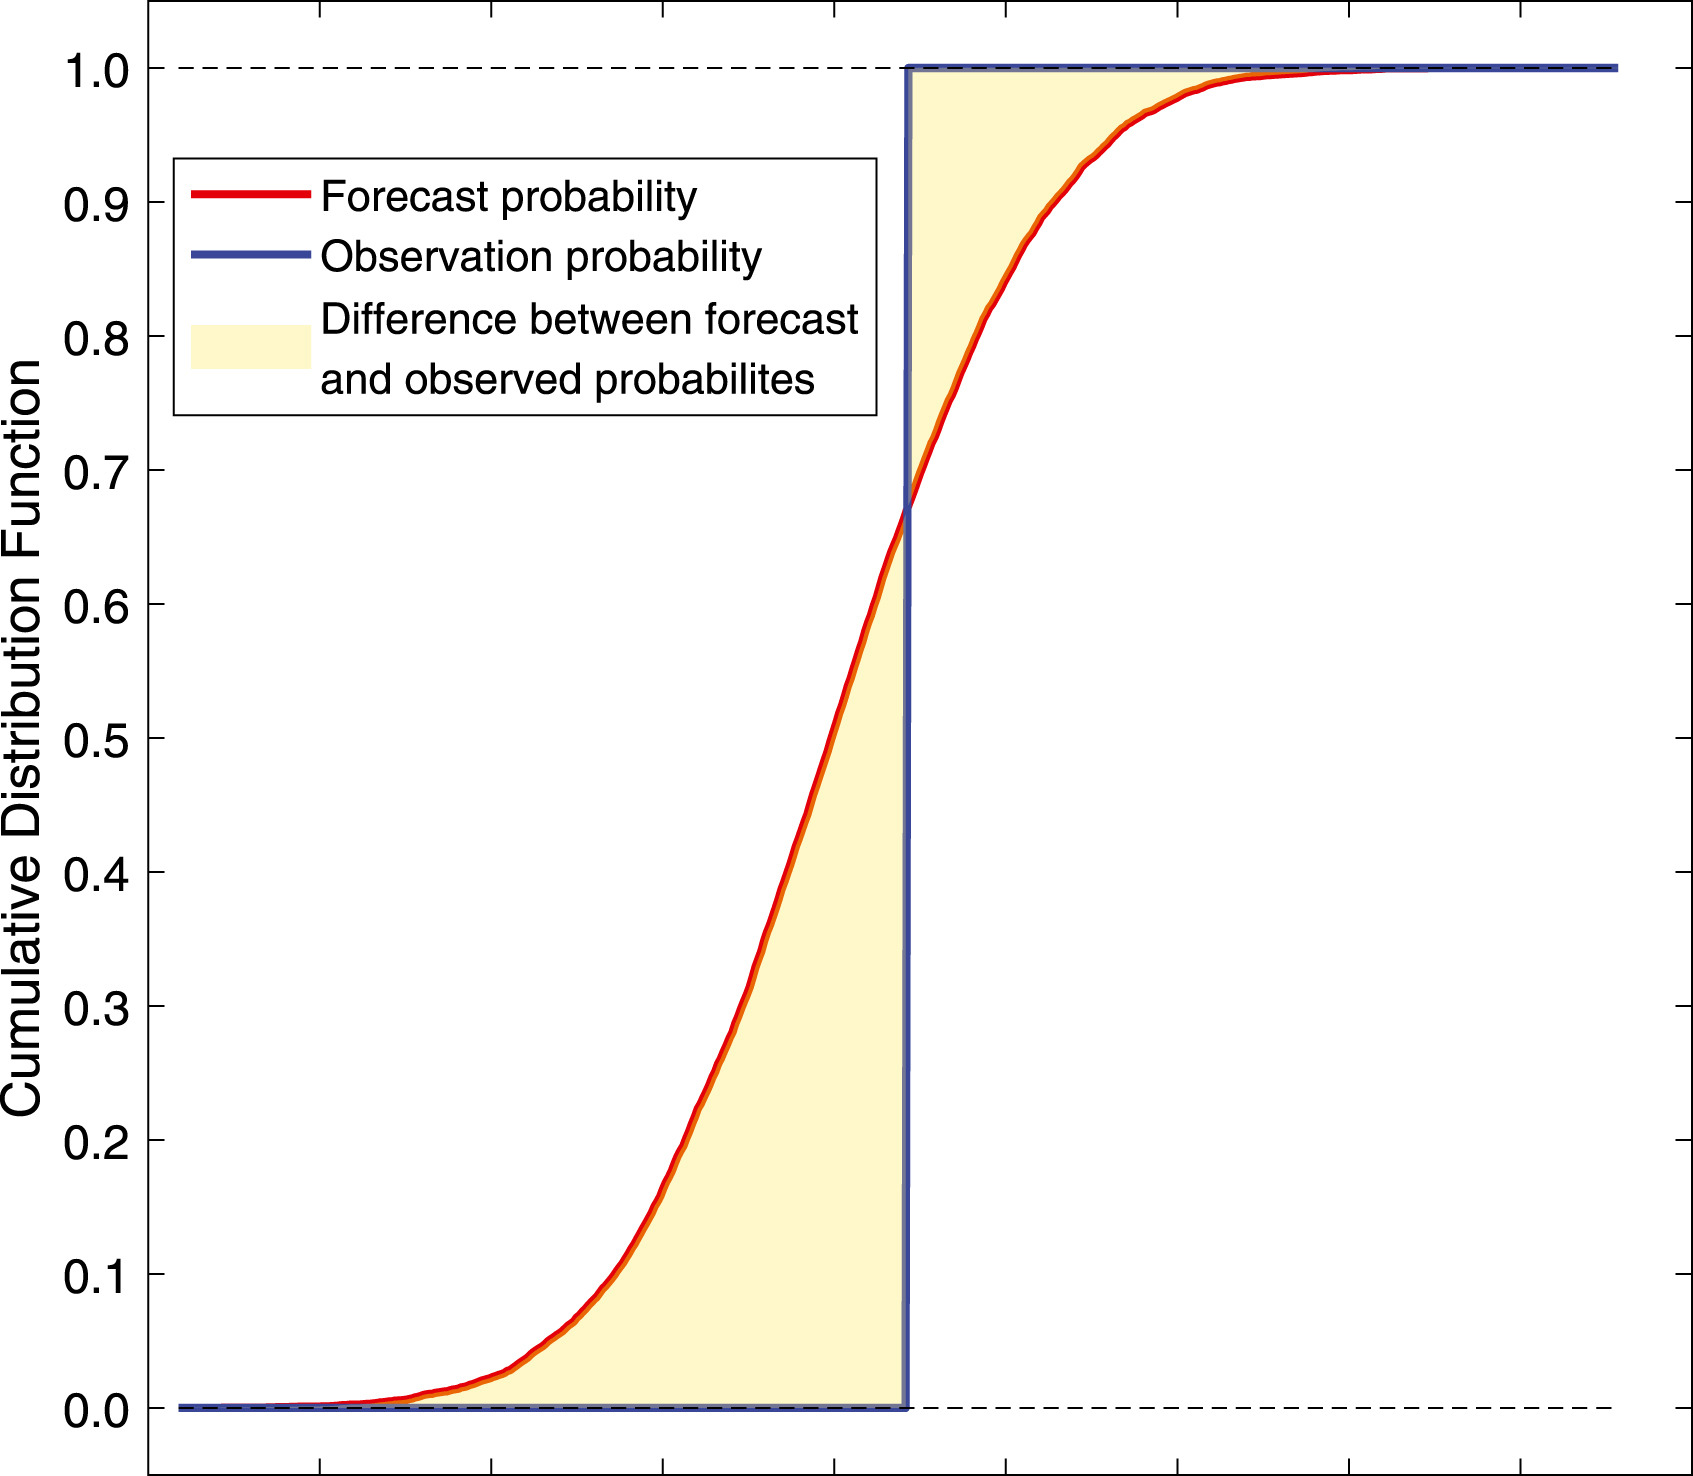
\includegraphics[width=0.6\linewidth,height=\textheight,keepaspectratio]{figs/crps.jpg}
\end{center}
\end{frame}

\begin{frame}[fragile]{Quantile score and CRPS}
\protect\phantomsection\label{quantile-score-and-crps}
\fontsize{11}{12}\sf

\begin{Shaded}
\begin{Highlighting}[]
\NormalTok{beer\_fc }\SpecialCharTok{|\textgreater{}}
  \FunctionTok{accuracy}\NormalTok{(aus\_production, }\FunctionTok{list}\NormalTok{(}\AttributeTok{measures=}\NormalTok{distribution\_accuracy\_measures))}
\end{Highlighting}
\end{Shaded}

\begin{verbatim}
# A tibble: 2 x 4
  .model .type measures.percentile measures.CRPS
  <chr>  <chr>               <dbl>         <dbl>
1 mean   Test                22.7          22.4 
2 snaive Test                 8.80          8.71
\end{verbatim}
\end{frame}

\begin{frame}[fragile]{Quantile score}
\protect\phantomsection\label{quantile-score-1}
\fontsize{11}{12}\sf

\begin{Shaded}
\begin{Highlighting}[]
\NormalTok{beer\_fc }\SpecialCharTok{|\textgreater{}}
  \FunctionTok{accuracy}\NormalTok{(aus\_production, }\FunctionTok{list}\NormalTok{(}\AttributeTok{qs=}\NormalTok{quantile\_score), }\AttributeTok{probs =}\NormalTok{ .}\DecValTok{9}\NormalTok{)}
\end{Highlighting}
\end{Shaded}

\begin{verbatim}
# A tibble: 2 x 3
  .model .type    qs
  <chr>  <chr> <dbl>
1 mean   Test  14.1 
2 snaive Test   4.60
\end{verbatim}
\end{frame}




\end{document}
